\hypertarget{ux434ux43e-ux441ux432ux438ux434ux430ux43dux438ux44f-russie}{%
\section{До свидания, Russie
!}\label{ux434ux43e-ux441ux432ux438ux434ux430ux43dux438ux44f-russie}}

\emph{Samedi 09 juin 2018}

Le temps file à vive allure. Et il nous amène déjà à notre prochaine
destination. Nous avons donc passé nos deux derniers jours à dire
au-revoir à nos amis russes en festoyant, tout en gardant pour la fin de
notre séjour une visite au musée Pouchkine.

\begin{figure}
\centering
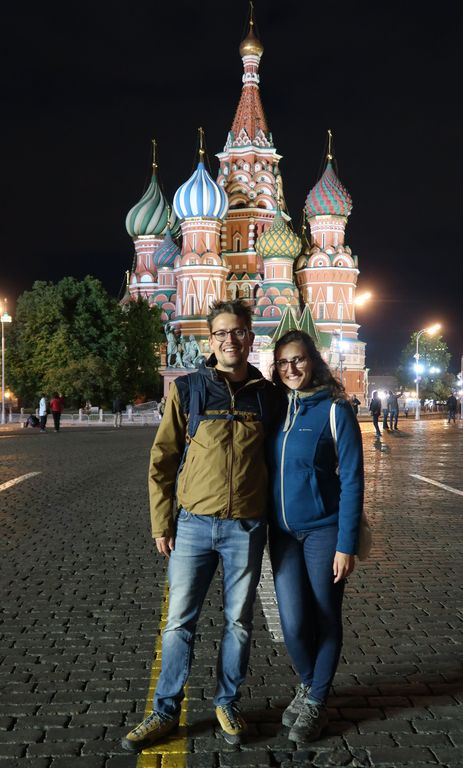
\includegraphics{images/20180609_aurevoir.JPG}
\caption{Souvenir du dernier soir : la place Rouge et la cathédrale de
Basile.}
\end{figure}

Pourquoi cette visite ? Les lecteurs attentifs de ce blog apprécieront :
inspirés par
\href{https://www.franceinter.fr/emissions/sur-les-epaules-de-darwin/sur-les-epaules-de-darwin-10-mars-2018}{une
récente émission de Jean-Claude Ameisen}, nous sommes allés voir le
"trésor de Priam" découvert lors des fouilles sur la côte turque par
Heinrich Schliemann à la fin du XIXème siècle. Cédé à un musée berlinois
par l'archéologue, le trésor avait disparu lors de la prise de
l'Allemagne en 1945 par l'union soviétique. Et comme l'histoire a
souvent plus d'un tour dans son sac, ce trésor est réapparu dans les
années 90 à Moscou. Cette anecodote racontée lors de l'émission était
trop belle pour rater cette visite. D'autant plus que le musée présente
également de belles tablettes mésopotamiennes...

Avant de nous diriger vers l'aéroport qui va nous emmener en Russie,
nous faisons le tour des stations de métro sur la ligne circulaire de
Moscou et admirons une dernière fois la diversité et la qualité de cet
endroit. Direction : la Chine !

\emph{Florian et Elida}
